\chapter{提案手法の統合}

\section{提案手法}

これまでに説明してきた手法の中で,検索性能の向上に有効な結果を示したものを統合し,検索精度の更なる向上を図る.検索性能の向上に有効な結果を示したものとして,論文の利用・Kaldiを用いた検索文書の利用・キャッシュモデル・前後の部分文書の情報を加味の手法があり,これらを統合し,検索精度の変化を分析する.

\subsection{実験条件}
実験条件を表\ref{t_ex_patern}に示す.

\begin{table}[h]
    \centering
    \caption{実験条件}
    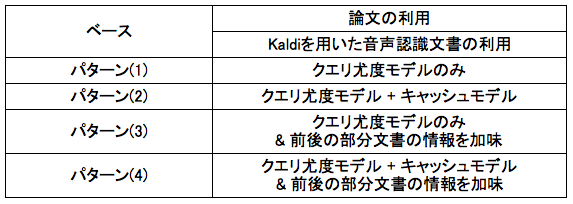
\includegraphics[width=7cm]{./image/t_ex_patern.png}
    \label{t_ex_patern}
\end{table}
実験は,表\ref{t_condition1}と同様に,NTCIR11 SpokenQuery\&Doc Formal-run の SQSCR SGS Retrieval条件で行った.
基本的に,論文の利用とKaldiを用いた検索文書を用い,パターン(1) クエリ尤度モデルのみ, パターン(2) キャッシュモデルの2つのパターンについて,変化させたときのMAP値を算出する.
また,2つのパターンのそれぞれに対し,前後の部分文書の情報を加味をした4パターンについて比較,分析した.



\subsection{実験結果}

\begin{table}[htbp]
    \centering
    \caption{提案手法を統合したときのMAP値}
    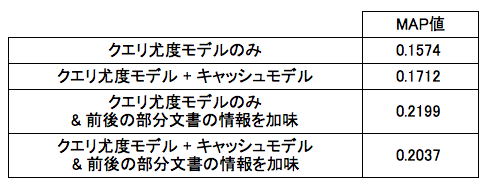
\includegraphics[width=7cm]{./image/t_integration.png}
    \label{t_integration}
\end{table}

実験を行った結果を表\ref{t_integration}に示す.表\ref{t_integration}から,パターン(1)とパターン(2)において,それぞれに前後の部分文書の情報を加味した場合,MAP値は大幅に改善した.しかし,パターン(2)は,パターン(1)よりMAP値が大きいにも関わらず,前後の部分文書情報を加味したパターン(4)はパターン(3)よりもMAP値が大きくならなかった.これは,キャッシュモデルがすでに検索対象文書の出現場所以前の情報を保持しているため,前後の部分文書情報を加味した場合に重複した特徴量となってしまい,MAP値が低下するのではないかと考えられる.

% TODO: パラメータの説明もメモしといた方が良い